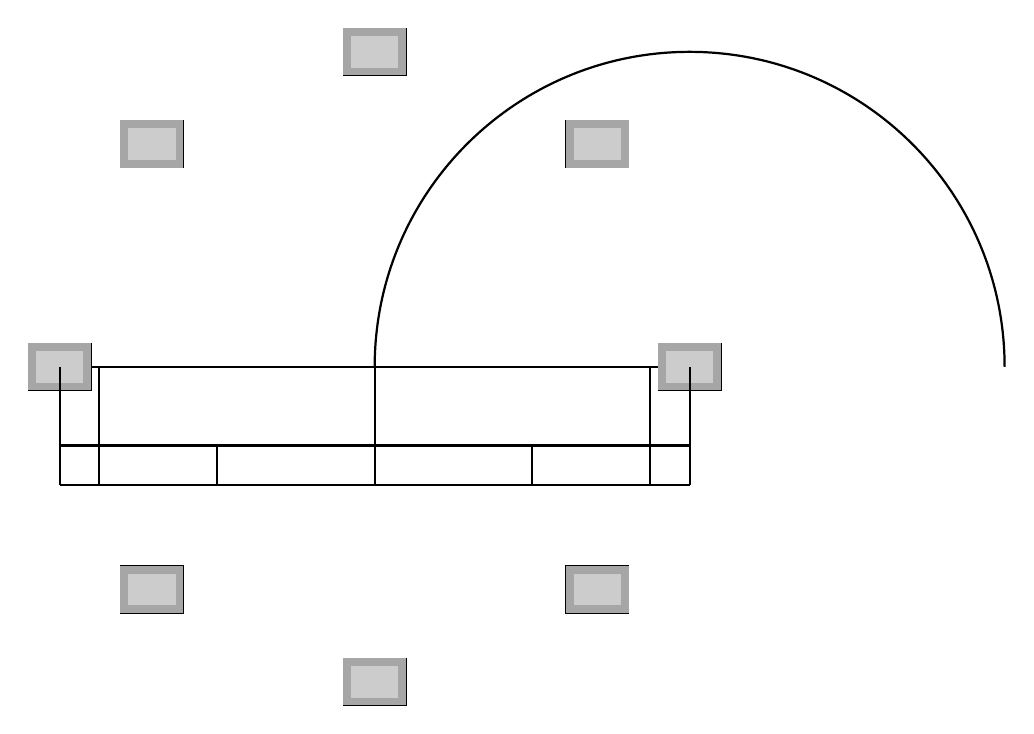
\begin{tikzpicture}
% Define the arch parameters
\def\archRadius{4} % radius of the arch
\def\archSpan{8}   % span of the arch (width at the base)
\def\deckHeight{1} % height of the deck
\def\stoneWidth{0.8} % width of each stone
\def\stoneHeight{0.6} % height of each stone
\def\numStones{8} % number of stones along the arch

% Draw the arch outline
\draw[thick] (0,0) arc[start angle=180, end angle=0, radius=\archRadius];
% Draw the base of the arch
\draw (-\archSpan/2,0) -- (\archSpan/2,0);

% Draw the stones along the arch
\foreach \i in {1,...,\numStones} {
    % Calculate the position along the arch
    \pgfmathsetmacro{\angle}{180 - (\i-1)*360/\numStones} % from 180 to 0 degrees
    \pgfmathsetmacro{\x}{\archRadius*cos(\angle)}
    \pgfmathsetmacro{\y}{\archRadius*sin(\angle)}
    % Draw the stone as a rectangle following the arch's curve
    % Maybe adjust the position to be centered on the arch's curve
    \draw[fill=gray!50] (\x - \stoneWidth/2, \y - \stoneHeight/2) rectangle (\x + \stoneWidth/2, \y + \stoneHeight/2);
}

% Draw the bridge deck
\draw[thick] (-\archSpan/2, -\deckHeight) rectangle (\archSpan/2, 0);

% Draw the supports (piers) from the deck to the arch
\foreach \i in {1,...,2} {
    \pgfmathsetmacro{\x}{-\archSpan/2 + (\i-1)*\archSpan/2} % left and right supports
    \draw[thick] (\x, -\deckHeight) -- (\x, 0);
}

% Draw the railing on the deck
\draw[thick] (-\archSpan/2, -\deckHeight) -- (-\archSpan/2, -\deckHeight - 0.5);
\draw[thick] (\archSpan/2, -\deckHeight) -- (\archSpan/2, -\deckHeight - 0.5);
\draw[thick] (-\archSpan/2, -\deckHeight - 0.5) -- (\archSpan/2, -\deckHeight - 0.5);
\draw[thick] (-\archSpan/2 + 0.5, -\deckHeight - 0.5) -- (-\archSpan/2 + 0.5, -\deckHeight);
\draw[thick] (\archSpan/2 - 0.5, -\deckHeight - 0.5) -- (\archSpan/2 - 0.5, -\deckHeight);
\foreach \i in {1,...,3} {
    \draw[thick] (-\archSpan/2 + \i*\archSpan/4, -\deckHeight - 0.5) -- (-\archSpan/2 + \i*\archSpan/4, -\deckHeight);
    \draw[thick] (\archSpan/2 - \i*\archSpan/4, -\deckHeight - 0.5) -- (\archSpan/2 - \i*\archSpan/4, -\deckHeight);
}

% Add some shading to the arch stones for depth
\foreach \i in {1,...,\numStones} {
    \pgfmathsetmacro{\angle}{180 - (\i-1)*360/\numStones}
    \pgfmathsetmacro{\x}{\archRadius*cos(\angle)}
    \pgfmathsetmacro{\y}{\archRadius*sin(\angle)}
    \fill[gray!70] (\x - \stoneWidth/2, \y - \stoneHeight/2) rectangle (\x + \stoneWidth/2, \y + \stoneHeight/2);
    % Add a slight shadow
    \fill[gray!40] (\x - \stoneWidth/2 + 0.1, \y - \stoneHeight/2 + 0.1) rectangle (\x + \stoneWidth/2 - 0.1, \y + \stoneHeight/2 - 0.1);
}

% Add the abutments at the ends of the arch
\draw[thick] (-\archSpan/2, 0) -- (-\archSpan/2, -1) -- (-\archSpan/2 + 0.5, -1) -- (-\archSpan/2 + 0.5, 0);
\draw[thick] (\archSpan/2, 0) -- (\archSpan/2, -1) -- (\archSpan/2 - 0.5, -1) -- (\archSpan/2 - 0.5, 0);

\end{tikzpicture}